\section{Концепция безопасности БД}

\subsection{Понятие безопасности БД}
Для того чтобы иметь общую точку старта нам придется дать пару определений, я постараюсь быстро разобраться с обязательной копипастой и перейти к делу. Итак:

\begin{grayquote}
	\textbf{База данных}\footnotemark -- это организованная коллекция данных, обычно хранящихся и доступных в электронном виде из компьютерной системы. Там, где базы данных более сложны, они часто разрабатываются с использованием формальных методов проектирования и моделирования.
\end{grayquote}

\begin{grayquote}
	\textbf{Система управления базами данных (СУБД)}\footnotemark[\value{footnote}] -- это программное обеспечение, которое взаимодействует с конечными пользователями, приложениями и самой базой данных для сбора и анализа данных. Программное обеспечение СУБД дополнительно включает в себя основные средства, предоставляемые для администрирования базы данных. Общая сумма базы данных, СУБД и связанных приложений может называться «системой базы данных». Часто термин «база данных» также используется для обозначения любой СУБД, системы баз данных или приложения, связанного с базой данных.
\end{grayquote}

Но если вас вдруг спросят, то смело отвечайте:
\begin{grayquote}
	Согласно \href{http://www.consultant.ru/cons/cgi/online.cgi?rnd=77B9A55845722924B47D00E78BFA3E50\&req=doc\&base=LAW\&n=329334\&dst=100282\&fld=134#2e1eph4wwt8}{гражданскому кодексу} Российской Федерации (часть четвертая) от 18.12.2006 N 230-ФЗ (ред. от 18.07.2019), базой данных является представленная в объективной форме совокупность самостоятельных материалов (статей, расчетов, нормативных актов, судебных решений и иных подобных материалов), систематизированных таким образом, чтобы эти материалы могли быть найдены и обработаны с помощью электронной вычислительной машины (ЭВМ).
\end{grayquote}

\footnotetext{Нагло скопипизженно с \href{https://en.wikipedia.org/wiki/Database}{вечно загнивающей}}

И если с просто базами данных все более-менее понятно, то в тот момент, когда нам приходиться говорить о вопросах безопасности, все превращается в классическую задачу о двух стульях: как надо и как в законе написано. (Ну или пафосно перефразируя) Вопросы информационной безопасности баз данных целесообразно рассматривать с двух взаимодополняющих позиций \autocite{Lihonosov2011}\footnote{Мне стыдно указывать ресурс, где я взял этот кусок, так что пусть будет \href{http://www.e-biblio.ru/book/bib/01_informatika/b_baz_dan/sg.html\#_Toc327430692}{pornhub}}:
\begin{itemize}
	\item оценочные стандарты, направленные на классификацию информационных систем и средств их защиты по требованиям безопасности
	\item технические спецификации, регламентирующие различные аспекты реализации средств защиты
\end{itemize}

Попытка защищать все и сразу обречена на провал, так что довольно логичным кажется сосредоточится на обеспечении безопасности четырех уровней информационной системы \autocite{Lihonosov2011}~\label{pon:urov}:
\begin{enumerate}
	\item уровня прикладного программного обеспечения, отвечающего за взаимодействие с пользователем
	\item уровня системы управления базами данных, обеспечивающего хранение и обработку данных информационной системы
	\item уровня операционной системы, отвечающего за функционирование СУБД и иного прикладного программного обеспечения
	\item уровня среды доставки, отвечающего за взаимодействие информационных серверов и потребителей информации
\end{enumerate}

Теперь уже можно ввести недостающие определения. Я вижу как вы соскучились по определениям\footnote{А эти определения я взял с прошлого года}.
\begin{grayquote}
Если БД рассматривать только как совокупность данных, то можно использовать следующее определения:
\begin{itemize}
	\item \textbf{Безопасность информации [данных]}: Состояние защищенности информации [данных], при котором обеспечены ее [их] конфиденциальность, доступность и целостность.
	\item \textbf{Информационная система (ИС)} -- система, предназначенная для хранения, поиска и обработки информации, и соответствующие организационные ресурсы (человеческие, технические, финансовые и т. д.), которые обеспечивают и распространяют информацию.
\end{itemize}

Если БД рассматривать как информационную систему, то можно использовать следующие определения:
\begin{itemize}
	\item \textbf{Безопасность ИС (БД)} можно определить как состояние защищенности ИС от угроз ее нормальному функционированию. Под защищенностью понимается наличие средств ИС и методов их применения, обеспечивающих снижение или ликвидацию негативных последствий, связанных с реализацией угроз. Изложенный подход к определению понятия безопасности ИС предполагает, что перечень и содержание угроз достаточно хорошо определены и достаточно стабильны во времени.

	\item \textbf{Безопасность ИС (БД)} можно определить как свойство системы адаптироваться к агрессивным проявлениям среды, в которой функционирует система, обеспечивающее поддержку на экономически оправданном уровне характеристики качества системы. В сформулированном определении основной акцент делается не на перечне и содержании угроз, нейтрализация которых обеспечивается, а на особую характеристику качества системы. При этом основной критерий качества ИС является экономическим, т.е. оценка средств и методов обеспечения безопасности осуществляется на основе затрат на реализацию механизмов безопасности и потенциальных выгод от недопущения ущерба, связанного с целенаправленным или случайным агрессивным проявлением среды.
\end{itemize}
\end{grayquote}

Ну и не одно введение не может обойтись без заклинания
\begin{grayquote}
	Проблема обеспечения безопасности автоматизированных информационных систем может быть определена как решение трех взаимосвязанных задач по реализации требуемого уровня:
	\begin{itemize}
		\item \textbf{конфиденциальности} -- обеспечения пользователям доступа только к данным, для которых пользователь имеет явное или неявное разрешение на доступ
		\item \textbf{целостности} -- обеспечения защиты от преднамеренного или непреднамеренного изменения информации или процессов ее обработки
		\item \textbf{доступности} -- обеспечения возможности авторизованным в системе пользователям доступа к информации в соответствии с принятой технологией
	\end{itemize}
\end{grayquote}

\subsection{Угрозы безопасности БД: общие и специфичные}
Интуитивное понимание угрозы безопасности можно сформулировать как нарушение великолепной тройки: \sout{Трус, Балбес и Бывалый} конфиденциальность, целостность, доступность. Для формального диалога можно использовать что-то около\footnote{Нагло взято \href{https://studopedia.su/2_30378_ugrozi-informatsionnoy-bezopasnosti-baz-dannih.html}{отсюда}}:
\begin{grayquote}
\textbf{Угрозой информационной безопасности} автоматизированный информационной системе (АИС) назовем возможность воздействия на информацию, обрабатываемую в системе, приводящего к искажению, уничтожению, копированию, блокированию доступа к информации, а также возможность воздействия на компоненты информационной системы, приводящего к утрате, уничтожению или сбою функционирования носителя информации или средства управления программно-аппаратным комплексом системы.
\end{grayquote}

Для того, чтобы разобраться во всем зоопарке перечисленных воздействий на систему нам придется все это дело классифицировать. Для удобства будем сразу смотреть на это со стороны обороняющего, то есть по источнику воздействия. В этом контексте они довольно естественно разбиваются на внутренние и внешние. Для описания внешних угроз необходимо учитывать объекты воздействия. (Под объектами воздействия понимаются объекты, которые могут подвергнуться атакам или могут стать причиной их возникновения.) \autocite{Ytebov2008}

Внешними дестабилизирующими факторами, создающими угрозы безопасности функционированию систем баз данных и СУБД, являются:
\begin{itemize}
	\item умышленные, деструктивные действия лиц с целью искажения, уничтожения или хищения программ, данных и документов системы, причиной которых являются нарушения информационной безопасности защищаемого объекта
	\item искажения в каналах передачи информации, поступающей от внешних источников, циркулирующих в системе и передаваемой потребителям, а также недопустимые значения и изменения характеристик потоков информации из внешней среды и внутри системы~\label{pon:pot}
	\item сбои и отказы в аппаратуре вычислительных средств
	\item вирусы и иные деструктивные программные элементы, распространяемые с использованием систем телекоммуникаций, обеспечивающих связь с внешней средой или внутренние коммуникации распределенной системы баз данных
	\item изменения состава и конфигурации комплекса взаимодействующей аппаратуры системы за пределы, проверенные при тестировании или сертификации системы
\end{itemize}

Внутренними источниками угроз безопасности баз данных и СУБД являются:
\begin{itemize}
	\item системные ошибки при постановке целей и задач проектирования автоматизированных информационных систем и их компонент, допущенные при формулировке требований к функциям и характеристикам средств обеспечения безопасности системы
	\item ошибки при определении условий и параметров функционирования внешней среды, в которой предстоит использовать информационную систему и, в частности, программно-аппаратные средства защиты данных
	\item ошибки и несанкционированные действия пользователей, административного и обслуживающего персонала в процессе эксплуатации системы
	\item недостаточная эффективность используемых методов и средств обеспечения информационной безопасности в штатных или особых условиях эксплуатации системы
\end{itemize}

Если у вас разбегаются глаза, это нормально -- здесь перечислены атаки на всех уровнях~\label{pon:urovs}. Что за уровни? Напоминаю:
\begin{itemize}
	\item На уровне сети
	\begin{itemize}
		\item Activex-объект
		\item Интерфейсы: OLE DB, ADO, ODBC, JDBC
		\item Протоколы: TCP/IP, IPX/SPX, Named Pipes, Multiprotocol
		\item Рабочие станции
		\item Серверы
		\item Маршрут
		\item URL
	\end{itemize}
	\item На уровне ОС
	\begin{itemize}
		\item Аппаратное обеспечение
		\item Программное обеспечение
		\item Файлы базы данных
		\item Файлы журнала транзакций
		\item Файлы резервного копирования
		\item Transact-SQL, PLSQL
		\item Службы: MSSQLServer, SQLServerАgent, TNSListener и т. д.
	\end{itemize}
	\item На уровне БД
	\begin{itemize}
		\item Пользователи
		\item Роли
		\item Роли приложения
		\item Диаграммы
		\item Представления
		\item Таблицы
		\item Хранимые процедуры
		\item Определения по умолчанию
		\item Правила
		\item Функции
		\item Тип данных
	\end{itemize}
\end{itemize}

Дальше, также легко и непринужденно можно разбить все атаки на СУБД на:
\begin{enumerate}
	\item атаки на уровне ОС
	\item атаки на уровне сети
	\item атаки на уровне БД
\end{enumerate}
Атаки на ОС, в которых функционирует СУБД, возникают гораздо чаще, так как защитить ОС гораздо сложнее, чем СУБД. Это обусловлено тем, что число различных типов защищаемых объектов в современных ОС может достигать нескольких десятков, а число различных типов защищаемых информационных потоков -- нескольких сотен. Возможность практической реализации той или иной атаки на ОС в значительной мере определяется архитектурой и конфигурацией ОС. Тем не менее существуют атаки, которые могут быть направлены практически на любые ОС:
\begin{enumerate}
	\item Кража ключевой информации (паролей)
	\item Подбор пароля
	\item Сканирование жестких дисков компьютера
	\item Превышение полномочий
	\item Атаки класса <<Отказ в обслуживании>>
\end{enumerate}
Наиболее опасные атаки на СУБД исходят из сетей. На уровне сетевого
программного обеспечения возможны следующие атаки на СУБД:
\begin{enumerate}
	\item Прослушивание канала
	\item Перехват пакетов на маршрутизаторе
	\item Создание ложного маршрутизатора
	\item Навязывание пакетов
	\item Атаки класса <<Отказ в обслуживании>>
\end{enumerate}

Теперь спускаемся на уровень самой БД. Для простоты восприятия разобьем все кучкам угроз конфиденциальности, целостности и доступности(Опять же, согласно \autocite{Ytebov2008}):
\begin{itemize}
	\item К угрозам конфиденциальности информации можно отнести следующие~\label{ugr:conf}:
	\begin{enumerate}
		\item Инъекция SQL. Во многих приложениях используется динамический SQL -- формирование SQL-предложений кодом программы путем конкатенации строк и значений параметров. Зная структуру базы данных, злоумышленник может либо выполнить хранимую программу в запросе, либо закомментировать <<легальные>> фрагменты SQL-кода, внедрив, например, конструкцию UNION, запрос которой возвращает конфиденциальные данные. В последнее время злоумышленник может использовать специальные программы, автоматизирующие процесс реализации подобных угроз.

		\item Логический вывод на основе функциональных зависимостей. Пусть дана схема отношения: $R(A_1,\ldots,A_n)$. Пусть $U = \{A_1,\ldots,A_n\}, X ,Y$ -- подмножества из $U$. $X$ функционально определяет $Y$, если в любом отношении $r$ со схемой $R(A_1,\ldots,A_n)$ не могут содержаться два кортежа с одинаковыми значениями атрибутов из $X$ и с различными из $Y$. В этом случае имеет место функциональная зависимость, обозначаемая $X \Rightarrow Y$ . В реальных БД при наличии сведений о функциональных зависимостях злоумышленник может вывести конфиденциальную информацию при наличии доступа только к части отношений, составляющих декомпозированное отношение.

		\item Логический вывод на основе ограничений целостности. Для кортежей отношений в реляционной модели данных можно задать ограничения целостности -- логические условия, которым должны удовлетворять атрибуты кортежей. При этом ограничение целостности может быть задано в виде предиката на всем множестве атрибутов кортежа. В случае попытки изменить данные в таблице, СУБД автоматически вычисляет значение этого предиката, и в зависимости от его истинности операция разрешается или отвергается. Многократно изменяя данные и анализируя реакцию системы, злоумышленник может получить те сведения, к которым	у него нет непосредственного доступа. К этому виду угроз можно отнести также анализ значений первичных/вторичных ключей.

		\item Использование оператора UPDATE для получения конфиденциальной информации. В некоторых стандартах SQL пользователь, не обладая привилегией на выполнение оператора SELECT, мог выполнить оператор UPDATE со сложным логическим условием. Так как после выполнения оператора UPDATE сообщается, сколько строк он обработал, фактически пользователь мог узнать, существуют ли данные, удовлетворяющие этому условию.
	\end{enumerate}
	\item К угрозам  целостности информации, специфические для СУБД можно отнести следующие~\label{ugr:cel}:
	\begin{enumerate}
		\item С помощью SQL-операторов UPDATE, INSERT и DELETE можно изменить данные в СУБД. Опасность заключается в том, что пользователь, обладающий соответствующими привилегиями, может модифицировать все записи в таблице.
	\end{enumerate}
	\item К угрозам доступности для СУБД можно отнести следующие:
	\begin{enumerate}
		\item Использование свойств первичных и внешних ключей. В первую очередь отнесем сюда свойство уникальности первичных ключей и наличие ссылочной целостности. В том случае, если используются натуральные, а не генерируемые системой значения первичных ключей, может создаться такая ситуация, когда в таблицу невозможно будет вставить новые записи,	так как там уже будут записи с такими же значениями первичных ключей. Если в БД поддерживается ссылочная целостность, можно организовать невозможность удаления родительских записей, умышленно создав подчиненные записи.
		\item Блокировка записей при изменении. Заблокировав записи или всю таблицу, злоумышленник может на значительное время сделать ее недоступной для обновления.
		\item Загрузка системы бессмысленной работой. Злоумышленник может выполнить запрос, содержащий декартовое произведение двух больших отношений. Мощность декартового произведения двух отношений мощности $N_1$ и $N_2$ равна $N_1 \cdot N_2$. Это означает, что при выдаче злоумышленником запроса вида SELECT * FROM Tab1, Tab1 ORDER BY 1, где мощность отношения (количество строк в таблице Tab1) $N_1 = 10000$, мощность результирующего отношения будет $N = N^2_1 = 10000^2$. Вычисление соединения и сортировка результирующего отношения потребуют значительных ресурсов системы и отрицательно скажутся на производительности операций других пользователей.
		\item Использование разрушающих программных средств. Например, атака типа <<троянский конь>> -- запуск пользователями программ, содержащих код, выполняющий определенные действия, внедренный туда злоумышленником.
	\end{enumerate}
\end{itemize}

\subsection{Требования безопасности БД}
Если сильно постараться то, на основании угроз можно выделить следующий список требований к безопасности БД\footnote{За оригиналом \href{https://tproger.ru/articles/db-security-basics/}{сюда}}:
\begin{itemize}
	\item Функционирование в доверенной среде. Под доверенной средой следует понимать инфраструктуру предприятия и ее защитные механизмы, обусловленные политиками безопасности. Таким образом, речь идет о функционировании СУБД в соответствии с правилами безопасности, применяемыми и ко всем прочим системам предприятия

	\item Организация физической безопасности файлов данных. Требования к физической безопасности файлов данных СУБД в целом не отличаются от требований, применяемых к любым другим файлам пользователей и приложений

	\item Организация безопасной и актуальной настройки СУБД. Данное требование включает в себя общие задачи обеспечения безопасности, такие как своевременная установка обновлений, отключение неиспользуемых функций или применение эффективной политики паролей

	\item Безопасность пользовательского ПО. Сюда можно отнести задачи построения безопасных интерфейсов и механизмов доступа к данным

	\item Безопасная организация и работа с данными. Вопрос организации данных и управления ими является ключевым в системах хранения информации. В эту область входят задачи организации данных с контролем целостности и другие, специфичные для СУБД проблемы безопасности. Фактически эта задача включает в себя основной объем зависящих от данных уязвимостей и защиты от них
\end{itemize}

Но настало время отставить логику в сторону и поговорить \sout{на эльфийском} о юридических требованиях. В целом, в России пытаются регламентировать эту отрасль, но в основном это басни про <<кругом враги>>, <<безопасная безопасность>> и <<импортозамещать до потери пульса>>. Даже <<вертикаль власти>> не забыли [\autocite{Mysev2019}].\footnote{Если очень хочется, то можно преисполниться вот \href{https://publications.hse.ru/mirror/pubs/share/folder/ie7oj6cz00/direct/202314863}{этой монографией}}

Для беглого ознакомления достаточно заглянуть в
\href{http://www.consultant.ru/document/cons_doc_LAW_61798/0e9ec16b786dcbdaaa7f44abfc4a15e601d5be22/#dst100144}{ФЗ <<Об информации, информационных технологиях и о защите информации>>} и в \href{http://www.consultant.ru/document/cons_doc_LAW_75586/#dst0}{Указ президента <<О мерах по обеспечению информационной безопасности Российской Федерации при использовании информационно-телекоммуникационных сетей международного информационного обмена>>}. Хоть что-то более-менее содержательное начинается с \href{https://fstec.ru/en/288-tekhnicheskaya-zashchita-informatsii/obespechenie-bezopasnosti-kriticheskoj-informatsionnoj-infrastruktury/prikazy/1702-prikaz-fstek-rossii-ot-14-marta-2014-g-n-32}{требований ФСТЭК}.

Итак, согласно ФСТЭКу автоматизированная система управления, имеет многоуровневую структуру~\label{pon:bez}:
\begin{enumerate}
	\item уровень операторского (диспетчерского) управления (верхний уровень)
	\item уровень автоматического управления (средний уровень)
	\item уровень ввода (вывода) данных исполнительных устройств (нижний (полевой) уровень)
\end{enumerate}

В автоматизированной системе управления объектами защиты являются:
\begin{enumerate}
	\item информация (данные) о параметрах (состоянии) управляемого (контролируемого) объекта или процесса
	\item программно-технический комплекс, включающий технические средства, программное обеспечение, а также средства защиты информации
\end{enumerate}
\begin{grayquote}
	Принимаемые организационные и технические меры защиты информации:
	\begin{itemize}
		\item должны обеспечивать доступность обрабатываемой в автоматизированной системе управления информации (исключение неправомерного блокирования информации), ее целостность (исключение неправомерного уничтожения, модифицирования информации), а также, при необходимости, конфиденциальность (исключение неправомерного доступа, копирования, предоставления или распространения информации)

		\item должны соотноситься с мерами по промышленной, физической, пожарной, экологической, радиационной безопасности, иными мерами по обеспечению безопасности автоматизированной системы управления и управляемого (контролируемого) объекта и (или) процесса

		\item не должны оказывать отрицательного влияния на штатный режим функционирования автоматизированной системы управления.
	\end{itemize}
\end{grayquote}

\begin{grayquote}
	Организационные и технические меры защиты информации, реализуемые в автоматизированной системе управления в рамках ее системы защиты, в зависимости от класса защищенности, угроз безопасности информации, используемых технологий и структурно-функциональных характеристик автоматизированной системы управления и особенностей ее функционирования должны обеспечивать:
	\begin{itemize}
		\item идентификацию и аутентификацию (ИАФ)
		\item управление доступом (УПД)
		\item ограничение программной среды (ОПС)
		\item защиту машинных носителей информации (ЗНИ)
		\item аудит безопасности (АУД)
		\item антивирусную защиту (АВЗ)
		\item предотвращение вторжений (компьютерных атак) (СОВ)
		\item обеспечение целостности (ОЦЛ)
		\item обеспечение доступности (ОДТ)
		\item защиту технических средств и систем (ЗТС)
		\item защиту информационной (автоматизированной) системы и ее компонентов (ЗИС)
		\item реагирование на компьютерные инциденты (ИНЦ)
		\item управление конфигурацией (УКФ)
		\item управление обновлениями программного обеспечения (ОПО)
		\item планирование мероприятий по обеспечению безопасности (ПЛН)
		\item обеспечение действий в нештатных ситуациях (ДНС)
		\item информирование и обучение персонала (ИПО)
	\end{itemize}
\end{grayquote}

Для разнообразия можно ознакомиться с положением дел в Беларуси. Там есть вот такие прикольные законы\footnote{А это взято с \href{http://www.bseu.by/it/tohod/lekcii9_2.htm}{лекций по администрированию баз данных}}:
\begin{itemize}
	\item Об информатизации
	\item О научно-технической информации;
	\item О национальном архивном фонде и архивах в Республике Беларусь
	\item О печати и других средствах массовой информации
	\item О правовой охране программ для ЭВМ и баз данных
	\item О введении в действие Единой системы классификации и кодирования технико-
	экономической и социальной информации Республики Беларусь
	\item и др.
\end{itemize}

\subsection{Защита от несанкционированного доступа}
Когда мы начинаем говорить о безопасности бд, в первую очередь в голову приходит мысль, что не плохо было бы подумать о конфиденциальности (а уже потом про доступность и тд.). С нее и начнем.

К основным средствам защиты информации относят следующие\footnote{За оригиналом \href{https://refdb.ru/look/2755914.html}{сюда}}:
\begin{itemize}
	\item идентификация и аутентификации
	\item установление прав доступа к объектам БД
	\item защита полей и записей таблиц БД
	\item шифрование данных и программ
\end{itemize}

Простейший пример аутентификации это парольная защита. Парольная защита представляет простой и эффективный способ защиты БД от несанкционированного доступа. Пароли устанавлюваются конечным пользователями или администраторами БД и хранятся в определенных системных файлах СУБД в зашифрованном виде. Улучшенным вариантом является использование механизма SSL-аутентификации с использованием сертификатов.

В целях контроля использования основных ресурсов СУБД во многих системах имеются средства установления прав доступа к объектам БД. Права доступа определяют возможные действия над объектами. Владелец объекта, а также администратор БД имеют все права. Остальные пользователи к разным объектам могут иметь различные уровни доступа.

К данным, имеющимся в таблице, могут применяться меры защиты по отношению к отдельным полям и отдельным записям. В реляционных СУБД отдельные записи специально не защищаются. Применительно к защите данных в полях таблицы можно выделить такие уровни прав доступа, как полный запрет доступа, только чтение, разрешение всех операций (просмотр, ввод новых значений, удаление, изменение). Более мощным средством защиты данных является их шифрование. Для расшифрования информации пользователи, имеющие санкционированный доступ к зашифрованным данным, имеют ключ и алгоритм расшифрования.

Итак, для минимизации риска несанкционированного доступа необходима реализация комплекса нормативных, организационных и технических защитных мер, в первую очередь: введение ролевого управления доступа, организация доступа пользователей по предъявлению сертификата, выборочное шифрование для сегментов базы данных.

\subsection{Защита от вывода}
Мы уже говорили об этом в угрозах безопасности \ref{ugr:conf} на \pageref{ugr:conf} странице. У \autocite{Ytebov2008} есть только объяснение логического вывода на основе функциональных зависимостей или ограничений целостности, а за решением нас посылают в \autocite{Smirnov2007}. О! Я тут неожиданно понял что все, что я находил в интернете, в статьях и других книгах это копипаста различной степени наглости из \autocite{Smirnov2007}. Так что не буду отличаться оригинальностью и я. Помимо очевидного мониторинга с целью свести количество таких связей к минимуму, надо очень внимательно следить за привилегиями (принцип минимальных привилегий).
\begin{grayquote}
	Привилегия -- это разрешение на выполнение в системе определенного действия. Не имея соответствующей привилегии, пользователь не может получить доступ к данным или выполнить какое-либо действие.
\end{grayquote}

Все привилегии могут быть разделены на два класса: системные привилегии и привилегии доступа к объектам.

\begin{grayquote}
	Системная привилегия -- это привилегия, которая дает пользователю право на выполнение какой-либо операции в масштабе базы данных. Например, пользователь с системной привилегией ALTER TABLESPACE может изменять любую табличную область (за исключением некоторых ограничений на табличную область SYSTEM).

	Привилегия доступа к объекту -- это разрешение пользователю на выполнение определенной операции над определенным объектом, например выполнение выборки из некоторой таблицы.
	При этом пользователь может формировать любые запросы к данной таблице, но не имеет права модифицировать данные этой таблицы или формировать какой-либо запрос к другой таблице.
\end{grayquote}

\subsection{Целостность БД}
Когда мы говорили о защите от НСД, речь шла о конфиденциальности. Теперь настало время целостности.

По \autocite{Smirnov2007}:
\begin{grayquote}
	Задача обеспечения целостности предусматривает комплекс мер по предотвращению непреднамеренного изменения или унич­тожения информации, используемой информационной системой управления или системой поддержки принятия решений. Изменение или уничтожение данных может быть следствием неблагоприятного стечения обстоятельств и состояния внешней среды (стихийные бедствия, пожары и т. п.), неадекватных действий пользователей (ошибки при вводе данных, ошибки операторов и т. п.) и проблем, возникающих при многопользовательской обработке данных.

	Угроза нарушения целостности включает в себя любое умыш­ленное или случайное изменение информации, обрабатываемой в информационной системе или вводимой из первичного источника
	данных. К нарушению целостности данных может привести как преднамеренное деструктивное действие некоторого лица, изменяющего данные для достижения собственных целей, так и
	случайная ошибка программного или аппаратного обеспечения, приведшая к безвозвратному разрушению данных.
\end{grayquote}

Мы уже обсуждали основные угрозы целостности в \ref{ugr:cel} на \pageref{ugr:cel}.

Средства обеспечения целостности баз данных включают автоматическую поддержку некоторой системы правил, описывающих допустимость и достоверность хранимых и вводимых значений. Реляционная модель включает некоторые характерные правила, вытекающие из существа модели: ограничения домена и ограничения таблицы.
\begin{itemize}
	\item Целостность домена предполагает, что допустимое множество значений каждого атрибута является формально определенным. То есть существуют формальные способы проверки того, что конкретное значение атрибута в базе данных является допустимым. Строка не будет вставлена в таблицу, пока каждое из значений ее столбцов не будет находиться в соответствующем домене (множестве допустимых значений).
	\item Целостность таблицы означает, что каждая строка в таблице	должна быть уникальной. Хотя не все СУБД промышленного уровня требуют выполнения такого ограничения, возможность уникальной идентификации каждой строки представляется необходимой для большинства реальных приложений.
\end{itemize}

Ограничения целостности позволяют гарантировать, что требования к данным будут соблюдаться независимо от способа их загрузки или изменения. В большинстве СУБД предусмотрена поддержка следующих типов статических ограничений целостности\footnote{Немного другая точка зрения: https://studfiles.net/preview/6354061/page:55/ (Роскомнадзор будет ругаться, но вас это пугать не должно)}:
\begin{enumerate}
	\item ограничение на определенность значения атрибута (NOT NULL)
	\item ограничение на уникальность значения атрибутов (UNIQUE)
	\item ограничение -- первичный ключ
	\item ограничение -- внешний ключ
	\item ограничение целостности, задаваемое предикатом
\end{enumerate}

\subsection{Аудит безопасности}

\subsubsection{Определение}

Аудит информационной безопасности информационных систем — это процесс оценки системы защиты информации на предмет соответствия стандартам и требованиям безопасности, а также выявления уязвимостей и возможных угроз безопасности.

\subsubsection{Цели проведения аудита}

Основной целью проведения аудита информационной безопасности является выявление уязвимостей в системе защиты информации и предотвращение возможных угроз безопасности. Кроме того, аудит также позволяет определить эффективность системы защиты, а также проверить соответствие информационных систем законодательству и стандартам безопасности.

\subsubsection{Процесс проведения аудита}

Процесс проведения аудита обычно включает 3 этапа:
\begin{enumerate}
	\item Подготовка и планирование
	\item Аудит
	\item Отчет
\end{enumerate}

\paragraph{1. Подготовка и планирование.}

На этом этапе формируется команда, которая будет проводить аудит, определяется область аудита, составляется план и график проведения аудита.

Область аудита — это система, на которой будет сосредоточен аудит. Определяются приоритетные активы и периметр аудита. Связанные активы изучаются и классифицируются как находящиеся в периметре аудита или за его пределами. Определение области аудита требует от аудитора четкого понимания устройста инфраструктуры и организационной структуры. Список активов должен быть составлен путем анализа документации, архитектуры системы и организационных иерархий. Должны быть включены как материальные (например, компьютеры, серверы, принтеры, отдельные лица), так и нематериальные (например, данные, электронная почта, веб-приложения, пароли) элементы. Угрозы этим активам должны быть идентифицированы, а приоритизация осуществляется с использованием результатов анализа рисков. Хорошей практикой является проверка результатов предыдущего аудита безопасности, чтобы понять, какие приоритеты были расставлены в прошлом.

После определения области аудита можно четко определить цели аудита и составить план. План составляется с учетом уже собранной информации, а также с учетом даты и времени проведения аудита, стратегии резервного копирования и влияния процесса на ежедневные операции.

Из-за множества компонентов системы (например, файлов, серверов, приложений, данных) и методов (например, политик, межсетевых экранов, биометрии, шифрования), задействованных в обеспечении безопасности, практически невозможно провести аудит всей системы одновременно. Поэтому в разное время года для организации планируются несколько небольших аудитов безопасности, каждый из которых фокусируется только на определенной области. Обычная разбивка областей аудита безопасности включает в себя физическую безопасность, безопасность ОС, веб-приложений, веб-серверов, серверов БД, сетевого оборудования, политик и процедур.

График проведения аудита может сильно измениться, если резко меняются приоритеты. Например, в таблице на Рис. 1 представлен возможный график аудита безопасности для организации. В первом столбце таблицы отображается исходный график аудита, а во втором столбце отображается тот же график после внесения корректировок из-за обнаружения уязвимости (возможной SQL-инъекции).

\begin{figure}[h!]
    \centering
    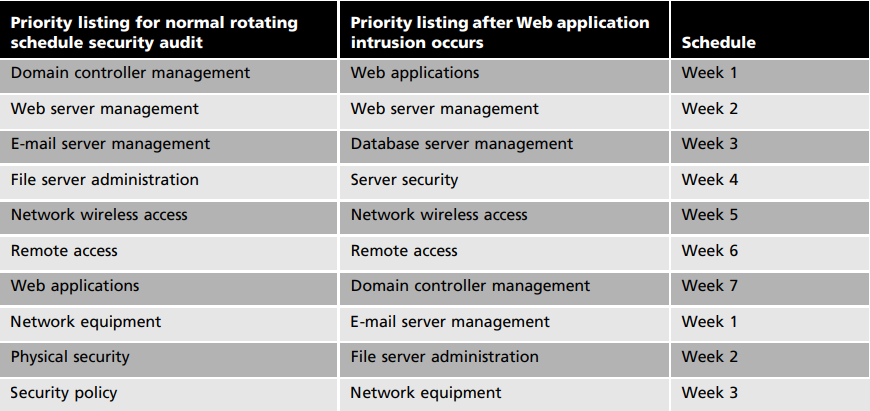
\includegraphics[width=0.8\textwidth]{assets/Schedule_audit}
    \caption{Пример графика проведения аудита}
\end{figure}

\paragraph{2. Аудит.}

На этом этапе подробный план аудита безопасности, составленный на предыдущем этапе, приводится в действие. Конкретные действия во время проведения аудита зависят от множества факторов, включая тип аудита, область аудита и организацию. Очевидно, что аудит, предназначенный для проверки физической безопасности, будет включать в себя совершенно иные действия, чем аудит, предназначенный для проверки администрирования СУБД. На Рис.2 в таблице показан список действий, которые обычно выполняются в процессе аудита для разных типов систем.

\begin{figure}[h!]
    \centering
    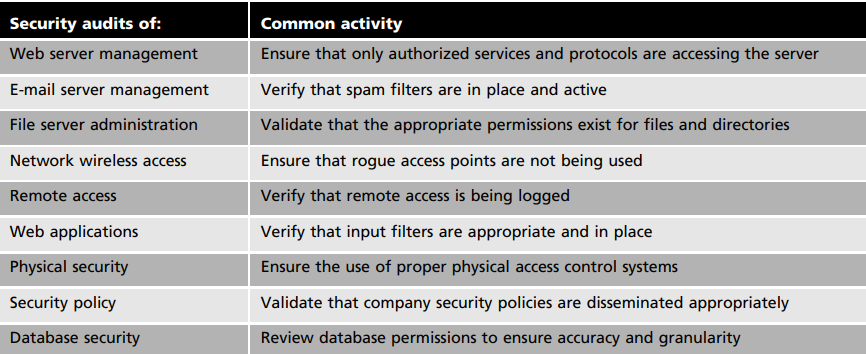
\includegraphics[width=0.8\textwidth]{assets/Common_actions_audit}
    \caption{Пример обычных действий при проведении аудита}
\end{figure}

\paragraph{3. Отчет.}

Заключительным этапом процесса аудита безопасности является подведение итогов, на котором аудитор или комитет аудиторов устно и письменно сообщает о результатах аудита.

Во всех аудиторских отчетах можно обнаружить некоторые важные общие черты, включающие исходную информацию, определенную область аудита, план и цель аудита, ключевые выводы, используемую для риск-аналитики методологию, рекомендации по устранению найденных уязвимостей.

\subsubsection{Процесс проведения аудита БД}

\paragraph{Подготовка и планирование аудита БД.}

Подготовка к аудиту безопасности БД требует, чтобы аудитор собрал как можно больше информации об инфраструктуре БД для четкого определения периметра аудита. Периметр должен включать подробную информацию о людях, данных, технологиях и документах, которые будут играть роль в рамках конкретного аудита. На Рис. 3 представлен пример периметра аудита БД.

Сбор информации включает в себя консультацию с администраторами БД, изучение схем баз данных, архитектуру сети, политик и процедур, связанных с БД. Часто организации имеют несколько СУБД, поэтому необходимо принять решение, сколько систем будет проверяться.

\begin{figure}[h!]
    \centering
    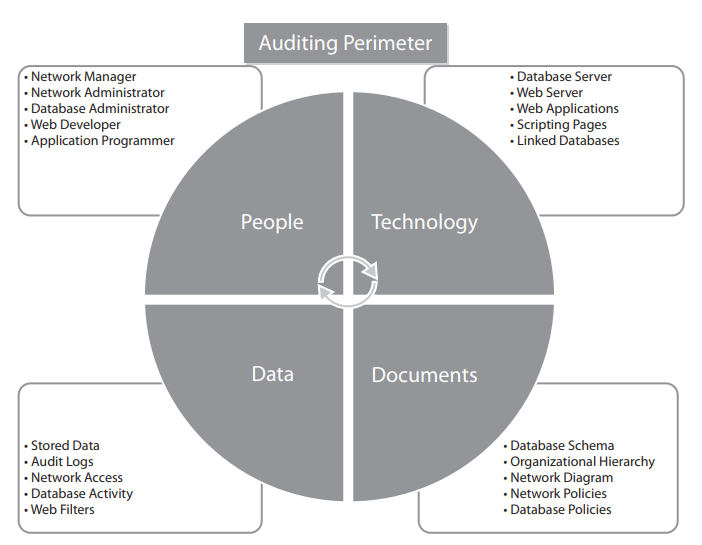
\includegraphics[width=0.8\textwidth]{assets/DB_audit_perimeter}
    \caption{Пример периметра аудита БД}
\end{figure}

На этом этапе также необходимо получить понимание функциональности, назначения и структуры всех используемых СУБД. Важна такая информация, как вендор СУБД, ОС функционирования СУБД, стратегия резервного копирования. Необходимо провести анализ данных на предмет связи с организационной иерархией, чтобы понять потребности сотрудников в хранении данных и манипулировании ими.

Анализ рисков и угроз является еще одним важным этапом планирования аудита БД, поскольку он помогает определить приоритетный список действий, который можно использовать в качестве отправной точки для аудита. Чтобы гарантировать, что были приняты все меры для защиты БД и учтены все риски, необходимо рассматривать всю инфраструктуру БД, в том числе сетевую.

Аудит БД может выполняться одним из двух способов. Аудитор может сначала сосредоточиться на компонентах, связанных с БД (например, веб-приложениях, веб-серверах, middleware, скриптах), прежде чем переходить к БД, или аудит может начаться с БД, и впоследствии проводится проверка связанных компонентов.

\paragraph{Аудит БД.}

Из-за большого количества ресурсов, необходимых для проверки всей инфрастуктуры БД, аудит обычно проводится частями, фокусируясь на конкретных функциях или компонентах. Эти части могут включать обслуживание серверов, администрирование учетных записей, контроль доступа, привилегии доступа к данным, пароли, шифрование, активность пользователей.

\paragraph{Обслуживание серверов.}

Аудит обслуживания сервера включает проверку стратегий резервного копирования, контроля обновлений и версий ПО, управления ресурсами и обновлениями оборудования. Ниже приведен список примеров аудиторских проверок:

\begin{enumerate}
	\item Установлены последние патчи безопасности СУБД
	\item Установлены последние критические обновления СУБД
	\item Используемая версия СУБД поддерживается
	\item Существует и используется процедура обновления СУБД
	\item Существует и применяется политика резервного копирования, включающая аварийное восстановление
	\item Существует и используется процедура проверки резервных копий
\end{enumerate}

\paragraph{Администрирование учетных записей.}

Аудит администрирования учетных записей включает проверку того, как администратор управляет учетными записями пользователей, а именно: создание, удаление учетных записей пользователей; применение политик безопасности; назначение групп, ролей и привилегий. Примеры аудиторских проверок:

\begin{enumerate}
	\item Различные роли администраторов четко определены
	\item Учетные записи администраторов распределяются согласно политике
	\item Неактивные или ненужные учетные записи пользователей удаляются
	\item Общие учетные записи не используются
	\item Учетные записи по умолчанию отключены или удалены
\end{enumerate}

\paragraph{Контроль доступа.}

Контроль доступа включает отслеживание доступа пользователей к БД. Контроль доступа необходим для обеспечения конфиденциальности, целостности и доступности СУБД. Примеры аудиторских проверок:

\begin{enumerate}
	\item Только доверенные IP-адреса могут получить доступ к базе данных
	\item Доступ к конфиденциальным данным имеют только те, кому они необходимы
	\item Администраторы не имеют возможности удаленно вносить изменения в БД без дополнительной аутентификации
	\item Доступ к резервным копиям и аварийному восстановлению разрешен только администраторам
\end{enumerate}

\paragraph{Привилегии доступа к данным.}

Обеспечение соответствия привилегий доступа во время аудита — трудоемкая задача, которая требует сотрудничества с сетевым администратором. Примеры аудиторских проверок:

\begin{enumerate}
	\item PUBLIC удален из системы
	\item Неявное предоставление привилегий тщательно рассматривается
	\item Используется принцип наименьших привилегий
	\item Привилегии учетной записи в операционной системе ограничены
\end{enumerate}

\paragraph{Пароли.}

Надежные пароли имеют решающее значение в доверенной среде, поскольку они представляют собой первую линию защиты, с которой столкнутся злоумышленники. Большинство СУБД можно настроить так, чтобы пароли автоматически соответствовали определенной политике. Аудит управления паролями включает проверку написанной политики, конфигурации сервера и учетных записей пользователей по умолчанию. Примеры аудиторских проверок:

\begin{enumerate}
	\item Опции управления паролями включены в СУБД
	\item Парольная политика включает спецификации для неудачных входов в систему, устаревания, сложности, истории, срока действия и содержимого
	\item Пароли по умолчанию должны быть изменены
	\item По возможности пароли не хранятся в БД
	\item Пароли шифруются с использованием стойкого шифрования, если они хранятся в БД
\end{enumerate}

\paragraph{Шифрование.}

Шифрование должно быть проверено как для хранящихся, так и для перемещаемых данных по БД. Примеры аудиторских проверок:

\begin{enumerate}
	\item Перемещаемые данные шифруются с использованием надежных методов шифрования
	\item Для шифрования данных используются симметричные ключи
	\item Шифрование настроено точно согласно политике
\end{enumerate}

\paragraph{Активность пользователей.}

Должен быть настроен мониторинг действий пользователей, работающих с СУБД. Примеры аудиторских проверок:

\begin{enumerate}
	\item Неудачные входы отслеживаются
	\item Неудачные запросы отслеживаются
	\item Изменения метаданных отслеживаются
\end{enumerate}

\paragraph{Отчет об аудите БД.}

Подготовка и презентация отчета об аудите БД совпадает с описанным ранее общим этапом аудита безопасности.

\begin{figure}[b]
Данный подразрадел является переводом и резюме 9 главы книги Database Security Альфред Баста и Мелисса Згола 2011 \href{https://pdfcoffee.com/alfred-basta-melissa-zgola-database-security-cengage-learning-2011-pdf-pdf-free.html}{ссылка на pdf}
\end{figure}

\clearpage

\subsection{Многоуровневая защита}
Мы уже успели поговорить про уровни в связке интерфейс-СУБД-ОП-среда [\ref{pon:urov}],  сеть-ОС-БД [\ref{pon:urovs}] и даже ФСТЭКовские уровни [\ref{pon:bez}].

Самое полное описание, пожалуй, сеть-ОС-БД, так что дальше будем отталкиваться от него. Вполне очевидно что защищать все и сразу сложно, каждый уровень имеет свою специфику, но какие то общие принципы выделить можно. Так как все труды на эту тему каскадно ссылаются на \autocite{Smirnov2007}, то просто процитирую:
\begin{grayquote}
	Анализ наиболее успешных решений в области обеспе­чения информационной безопасности баз данных позволил сформулировать несколько полезных принципов, которыми можно руководствоваться при проектировании систем защиты:
	\begin{itemize}
		\item экономическая оправданность механизмов защиты
		\item открытое проектирование
		\item распределение полномочий между различными субъектами в соответствии с правилами организации
		\item минимально возможные привилегии для пользователей и администраторов
		\item управляемость системы при возникновении отказов и сбоев
		\item психологическая приемлемость работы средств защиты данных
	\end{itemize}
\end{grayquote}

\subsection{Типы контроля безопасности: потоковый, контроль вывода, контроль доступа}
Про все три типа мы уже успели поговорить. В частности \ref{pon:pot} и \ref{pon:bez}. Единственное, что осталось уточнить -- это контроль доступа. Идейно он этот вопрос распадается на два: \textit{кому} и \textbf{что} мы будем разрешать?

\paragraph{Кому?}

Получение доступа к ресурсам информационной системы предусматривает выполнение трех процедур: идентификации, аутентификации и авторизации.

Общепринято, что технологии идентификации и аутентификации являются обязательным элементом защищенных систем, так как обеспечивают аксиоматический принцип персонализации субъектов и, тем самым, реализуют первый (исходный) программ­но-технический рубеж защиты информации в компьютерных системах.

Под идентификацией понимается различение субъектов, объектов, процессов по их моделям, существующим в форме имен. Под аутентификацией понимается проверка и подтверждение подлинности образа идентифицированного субъекта, объекта, процесса. Как вытекает из самой сути данных понятий, в основе тех­нологий идентификации и аутентификации лежит идеология вероятностного распознавания образов, обуславливая, соответственно, принципиальное наличие ошибок первого и второго рода.
\begin{enumerate}
	\item Сущность процедуры идентификации состоит в назначении пользователю, т. е. объекту -- потребителю ресурсов сервера баз данных -- имени. Имя пользователя -- это некоторая уникальная метка, соответствующая принятым соглашениям именования и обеспечивающая однозначную идентификацию объекта реального мира в пространстве отображаемых объектов. С позиций ИС источники, предъявившие идентификатор, неразличимы.
	\item Сущность процедуры аутентификации состоит в подтверждении подлинности пользователя, представившего идентификатор.
	\item Сущность процедуры авторизации состоит в определении перечня конкретных информационных ресурсов, с которыми аутентифицированному пользователю разрешена работа.

\end{enumerate}
Процедуры идентификации, аутентификации и авторизации являются обязательными для любой защищенной ИС.

\paragraph{Что?}
В целом используют одну из трех моделей безопасности: дискреционная, мандатная и ролевая.
\begin{enumerate}
	\item Простейшая (одноуровневая) модель безопасности данных строится на основе дискреционного (избирательного) принципа разграничения доступа, при котором доступ к объектам осуществляется на основе множества разрешенных отношений доступа в виде троек -- <<субъект доступа -- тип доступа -- объект доступа>>.

	Наглядным и распространенным способом формализованного представления дискреционного доступа является матрица доступа, устанавливающая перечень пользователей (субъектов) и перечень разрешенных операций (процессов) по отношению к каждому объекту базы данных (таблицы, запросы, формы, отчеты).

	\item Мандатная модель доступа характерна для случая, когда возможность конкретных действий с данными или документами определяется внешним, обычно глобальным собственником информации. Исторически в роли такого глобального собственника чаще всего выступало государство. Основная идея мандатной модели доступа состоит в приписывании объектам и субъектам доступа меток. Если метки объекта и субъекта соответствуют (в некотором смысле), то субъект получает право на выполнение определенных действий с объектом. В роли метки, приписываемой субъектам в государственных структурах, выступает, например, форма допуска. В реляционной модели в качестве структуры, обладающей меткой, естественно выбрать кортеж.

	\item В основу ролевой модели положена идея принадлежности всех данных системы некоторой организации, а не пользователю, как в случае моделей дискреционного и мандатного доступа. В целом модель ориентирована на упрощение и обеспечение формальной ясности в технологии обеспечения политики безопасности системы. Управление доступом в ролевой модели осуществляется как на основе матрицы прав доступа для ролей, так и с помощью правил, регламентирующих назначение ролей пользователям и их
	активацию во время сеансов.

	В ролевой модели классическое понятие субъект разделяется на две части: пользователь и роль. Пользователь — это человек, работающий с системой и выполняющий определенные служебные обязанности. Роль -- это активно действующая в системе абстрактная сущность, с которой связан ограниченный, логически связанный набор привилегий, необходимых для осуществления определенной деятельности. (Самым распространенным примером роли явля­ется присутствующая почти в каждой системе учетная запись администратора (например, root для UNIX и Administrator для Windows), который обладает специальными полномочиями и может использоваться несколькими пользователями.

	Ролевая модель включает три компонента: модель отображения пользователь -- роль, модель отображения привилегия -- роль и модель отображения роль -- роль. Для упрощения логической структуры объектов управления вводится понятие иерархии ролей. Роль, входящая в иерархию, может включать другие роли, наследуя все привилегии включаемых
	ролей.
\end{enumerate}
\clearpage
